Docker ist ein Ökosystem das von der Firma \textbf{\textit{Docker, Inc.}} aufgebaut wird.
Die Firma wurde im Jahr 2013 gegründet und ist dabei schon sehr erfolgreich in dem was sie tut.

Docker wurde in drei Runden mit 11 Investoren auf 150 Millionen Dollar gefounded.

Die Firma Entwickelt die Software \textbf{\textit{Docker}} und sie betreibt auch einen Service der sich
\textbf{\textit{Docker Hub}} nennt. Zudem bietet sie mit ihren eigenen Datacenters die Möglichkeit
Docker Hub zu nutzen.

\section{Was ist Docker}

“\textit{Docker} ist eine Open-Source-Software, die beim Linux-Betriebssystem dazu verwendet werden
kann, Anwendungen mithilfe von Betriebssystem Virtuallisierung in Containern zu isolieren.
Dies vereinfacht einerseits die Bereitstellung von Anwendungen, weil sich Container, die
alle nötigen Pakete enthalten, leicht als Dateien transportieren und installieren lassen.
Andererseits gewährleisten Container die Trennung der auf einem Rechner genutzten Ressourcen,
sodass ein Container keinen Zugriff auf Ressourcen anderer Container hat.”\footnote{Siehe: \url{http://de.wikipedia.org/w/index.php?title=Docker_(Software)&oldid=142961470}}

Docker basiert auf einer ähnlichen Technologie wie Linux Containers (LXC).

\subsection{Was ist ein Docker Image}

Ein Docker Image ist mehr oder weniger ein Betriebsystem Image. Mit Docker kann man Docker Images
als .iso Dateien exportieren und importieren. Speziell bei Docker Images ist, dass sich ein diese
in Layers aufteilen, somit kann ich ein bestehendes Docker Image nehmen und mein eigenes darauf
aufbauen. Das ist meines Erachtens die grösste Stärke bei Docker, da man z.B. sein RHEL 7 Linux
perfekt aufsetzen und härten kann und das als Docker Image speichert. Danach kann man alle
weiteren Applikationen darauf aufbauen. Der Aufbau solcher Images kann man mittels einer
Scriptspache in Dockerfiles beschreiben und somit automatisieren.

\subsection{Was ist ein Docker Container}

Ein Docker Container ist eine Instanz eines Docker Images. Der Docker Container läuft
auf dem Host Betriebsystem, in dem auch die Docker Software läuft. Aus einem Docker Image
können beliebig viele Docker Container gestartet werden.

Die Dockersoftware kann beim starten eines Containers Umgebungsvariablen und Netzerkports
von aussen her setzten und somit den Kontext eines jeweiligen Containers bestimmen.

\section{Was ist Docker Hub}

“\textit{Docker Hub} ist ein Repository für Docker-Images. Es teilt sich in einen öffentlichen
und einen privaten Teil auf. Im öffentlichen Teil kann jeder Nutzer seine selbst erstellten
Images hochladen und damit anderen Nutzern zur Verfügung stellen. Außerdem gibt es mittlerweile
offizielle Images, z. B. von Linux-Distributoren. Im privaten Teil des Docker Hubs können
Benutzer ihre Docker Images hochladen und dadurch einfach z. B. firmenintern verteilen, ohne
dass diese damit sofort öffentlich auffindbar sind.

Die Hub Software wurde von Docker Inc. als Open-Source-Software veröffentlicht, sodass
man die Vorteile des Hubs nun auch nutzen kann, ohne die eigenen Images auf die Server
von Docker laden zu müssen.”\footnote{Siehe: \url{http://de.wikipedia.org/w/index.php?title=Docker_(Software)&oldid=142961470}}

Analog zu Nexus für Java Artefakte kann man Docker Hub einsetzen um Docker-Images
zu verwalten.

\section{Linux Container vs. Virtual Machines}

Jede virtuelle Maschine hat nicht nur seine Applikations Binaries die ca. 100 MB gross ist, sondern
auch die Binaries des gesamten Betriebsystems, das ca. 10 GB gross ist. Zudem läuft das Betriebsystem
komplett in seiner eigenen Instanz.

\begin{figure}[htbp]
  \begin{center}
    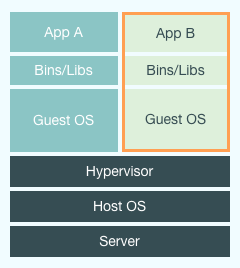
\includegraphics[width=0.45\textwidth]{./images/classic_virtual_machine.png}
    \caption{Klassiche Virtualisierung mit Host OS and Guest OS}
    \label{img:classic_virtual_machine}
  \end{center}
\end{figure}

Ein Linux Container läuft in einem eigenen Prozess im Host Betriebsystem. Der Linux Kernel isoliert
den Prozess von allen anderen Prozessen und mittels Namespaces. Das gibt die Vorteile einer
Virtuallisierung, ist aber viel leichtgewichtiger und Ressourcen schonender, da der Betriebsystem
overhead nur einmal anfällt.

\begin{figure}[htbp]
  \begin{center}
    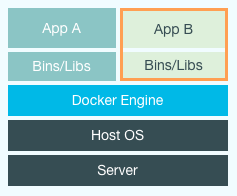
\includegraphics[width=0.45\textwidth]{./images/docker_container.png}
    \caption{Linux Container Virtuallisierung}
    \label{img:docker_container}
  \end{center}
\end{figure}




